

% \textbf{AL model}.
I was interested in looking at the behavior of a 2D system for the non-interacting case; a Gaussian packet lying entirely on the left side of the system was chosen as the initial state, and I also monitored the contrast $I(t)$. The presence of a global harmonic potential was described by a term of the form $\sum_j u_j \hat{n}_j$. Evolution was considered through ED (Exact Diagonalization) and expansion of the initial state into its own (fig. \ref{fig:2Dtherm}a). Similarly, at a small noise level the system was thermalized, and at large values it reached a localized state.

 
\begin{figure}[h]
    \centering
    \addletter{115}{a}
    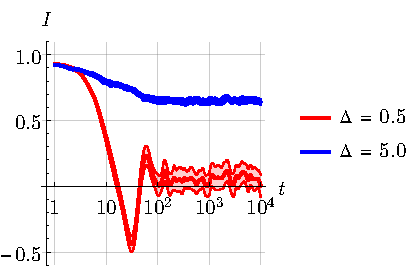
\includegraphics{imgs/2Dth_loc.pdf}
    % \hspace{5 mm} 
    \addletter{115}{b}
    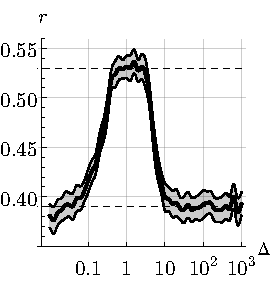
\includegraphics{imgs/2Drdel.pdf}
    % \hspace{5 mm} 
    \addletter{115}{c}
    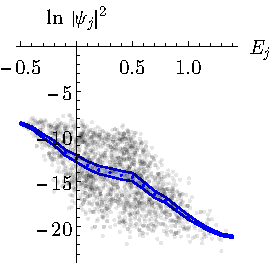
\includegraphics{imgs/2Dtherm_1.pdf}
    \caption{a) Evolution of contrast $I(t)$ averaged over 50 realizations $\delta_j$ for two noise levels $\Delta$: thermalization and localization. b) Dependence of $r$-parameter on the noise level $\Delta$, averaged over 50 realizations of $\delta_j$. c) For a thermalized state, the dependence of the population of the node $|\psi_j|^2$ on the energy of the node $E_j = \delta_j + u_j$, black dots indicate the dependence for a specific implementation $\delta_j$, blue indicates the result of averaging over 50 implementations.}
    \label{fig:2Dtherm}
\end{figure}



In the thermalizing state, the result is statistically significant and does not depend on the initial state (results not presented here). It is interesting to look at the resulting distribution of node population $\langle n_j\rangle_t$, averaged over time, from the energy of this node $\delta_j + u_j$ (fig. \ref{fig:2Dtherm}c). It is also interesting to compare $\langle n_j\rangle_t$ with the resulting thermal distribution $\tr n_j e^{-\beta H}$,  I obtained the correlation coefficient 
\begin{equation*}
    \text{corr}\,(\langle n_j\rangle_t, \tr n_j e^{-\beta H})|_{\Delta=0.5}  \approx 0.8,
    \hspace{10 mm} 
    \text{corr}\,(\langle n_j\rangle_t, \tr n_j e^{-\beta H})|_{\Delta=5}  \approx 0.2,
\end{equation*}
which is quite consistent with the ideas of localization and thermalization.




A natural question arises: how exactly can one characterize the localization phase and the ergodic phase (thermalizing) of a system, and what algorithm can be fed with the Hamiltonian. Various metrics are presented in \cite{pal_many-body_2010}, but the best place to start is the $r$-parameter, which is the focus of the next section.






% experimental implementation of the model

